\subsubsection{BinarySearchTree}
A Binary Search Tree(BST) tree is an evolved form of Binary Tree, that structured in a way that is more beneficial for storing large amounts of data. The criterias for a Binary tree to be a binary search tree is the following conditions:
\begin{itemize}
	\item{All left children nodes needs to have a value lower than its parent node.}
	\item{All right children nodes needs to have a value higher than its parent node.}
	\item{There cannot be any nodes with duplicate values in the tree.}
\end{itemize}
Having these requirements helps the BST search for the correct node, since the time it takes to find the correct node is shorten tremendously. Inserting new nodes in the tree is also quite simple, just traverse the tree, where the direction is dependent on the new nodes value. Once a leaf node has been reached, put it as either a left child or a right child based on whether the new node's value is lower or greater than the lead node's value.
\\[11pt]
The solution checker is designed to check that the tree object created from the students drawing, matches the tree created in the solution. The solution checker will recursively call a function named checkNode that will compare each node in the tree with the corresponding node in the solution. If the two nodes does not match, the solution checker will return false, and the student will have answered incorrect. If all nodes compared match the solution, the solution checker will return true, meaning that the student has answered the question correctly. The solution checker traverses the tree inorder. It will first check the left node, then the parent, then the right node. This solution checker is also used for AVL trees%Not 100percent certain anymore.
\\[11pt]
A function createBinarySearchTreeSolution was implemented to create a BST based on given arguments and/or existing tree object. This function was implemented so that the admin didn't need to manually create the solution trees for each question. The function takes an array with integers and possibly an existing tree as parameters. If the existing tree is not given, the function will create a new tree based on the values in the array. If the an existing tree is given, the values in the array is added to this tree. Its important to note that the function will not work with duplicate values in the array or given tree. \\
The createBinarySearchTreeSolution also needed to create resulting upon deleting an existing node in a tree. Because there are multiple ways to choose nodes for replacements when deleting a node with 2 children. It was required for the createBinarySearchTreeSolution to create a list of potential final resulting trees. It is required to specify whether the user wants to add nodes or remove nodes from the tree when creating the solution trees. The function cannot switch between the two during execution, and an existing tree is required in order to remove nodes in the tree.

%The image is currently not placed correctly, should wait until we mostly finished the content of the thesis.
\begin{figure}
	\centering
	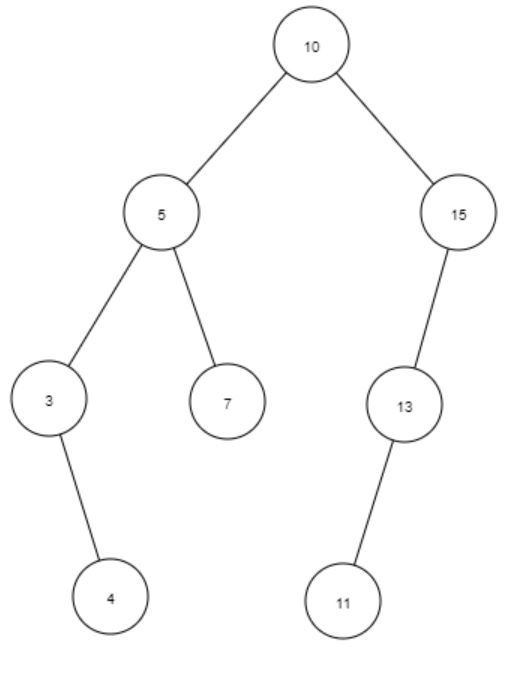
\includegraphics[width=250px, height=250px]{/trees/BST}
	\caption{The figure shows an example of a Binary Search Tree.}	
	\label{fig:BST}
\end{figure}
